\documentclass[12pt,a4paper, flushleft]{article}
\usepackage[utf8]{inputenc}
\usepackage{amsmath,amssymb,amsthm}
\usepackage[T2A]{fontenc}
\usepackage[russian]{babel}
\usepackage{mathrsfs, dsfont} % специальные шрифты, по типу \mathscr или \dsfont
\usepackage{comment} %для многострочных комментариев
\usepackage{xcolor} %для гиперссылок в тексте и их цвета
\usepackage{hyperref}
\usepackage{graphicx}
\usepackage{wrapfig}
\usepackage{lipsum}
\usepackage{multicol}
\graphicspath{/home/cowberry/Documents/10M/SPTYM/pics/}
\usepackage[left=2cm,right=2cm,top=2cm,bottom=2cm]{geometry}	
\usepackage[most]{tcolorbox}
\definecolor{block-gray}{gray}{0.90} % уровень прозрачности (1 - максимум)
\newtcolorbox{myquote}{colback=block-gray,grow to right by=-25mm,grow to left by=-25mm, boxrule=1pt,boxsep=0pt,breakable}
\author{Анатолий Коченюк, команда ЛНМО\#2}
\date{Март 2019}
\title{Зодача \textsuperscript{\textregistered} №5}
\newcommand{\horline}[1]{
		\begin{center}
			\begin{picture}(#1, 2)
				\line(1,0){#1}%
			\end{picture}
		\end{center}
	}
\title{
	\vspace{4cm}	
	\horline{470}	
	\begin{center}
		\begin{Huge}
			\textbf{\emph{Задача 1. Автостопом по галактике.}}
		\end{Huge}
	\end{center}	
	\vspace{-1.3cm}	
	\horline{480}
	%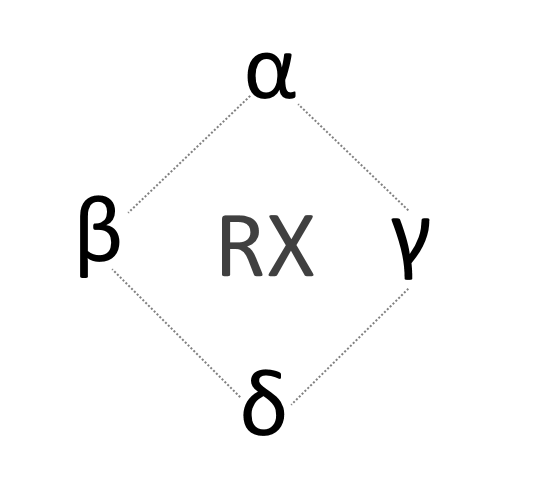
\includegraphics[scale=0.15]{abgrx.png}
}
\newtheorem{Def}{Определение}[section]
\newtheorem{Th}{Теорема}[section]
\newtheorem{Lm}{Лемма}[section] 
\newtheorem{Pb}{Задача}[section]
\newtheorem{Qu}{Признак}[section]
\newtheorem{St}{Утверждение}[section]
\newtheorem{Sl}{Следствие}[section]
\newtheorem{Zm}{Замечание}[section]
\newtheorem{Con}{Условие}[section]
\usepackage{relsize}
\newcommand{\vel}{\mathlarger{\mathlarger{\upsilon}}}
\newcommand{\der}[1]{\overset{\cdot}{#1}}
\newcommand{\dder}[1]{\overset{\cdot \cdot}{#1}}
\newcommand{\Lim}[2]{\lim\limits_{#1\to #2}}
\newcommand{\Ch}[1]{\overset{#1}{=}}
\newcommand{\p}[1]{#1^{\prime}}
\newcommand{\pp}[1]{#1^{\prime\prime}}
\newcommand{\ol}[1]{\overline{#1}}
\newcommand{\oll}[1]{\overline{\overline{#1}}}
\newcommand{\ov}[2]{\overset{#1}{#2}}
\newcommand{\un}[1]{\underline{#1}}
\newcommand{\gr}[2]{\includegraphics[scale=#1]{../pics/#2}}
\usepackage{comment}

\begin{document}
\maketitle

\pagebreak

\tableofcontents	
	
\pagebreak
\section*{Введение}

\begin{Def}
	Перестановка -- биективная функция $f: \mathds{Z}\to \mathds{Z}$
\end{Def}

\begin{Def}
	Перестановка $f$ называется конечной, если множество\\ $N_f = \{n\in\mathds{Z}\mid f(n)\neq n\}$ -- конечно.
\end{Def}

\begin{Def}
	Для $n\in\mathds{Z}$ множество $\mathcal{O}_f(n) = \{n, f(n), f(f(n))\dots\}\cup \{f^{-1}(n), f^{-1}(f^{-1}(n))\dots\}$ называется орбитой $n$ под действием $f$.
\end{Def}

\begin{Def}
	Перестановка $f$ называется локально конечной, если у всех $n\in\mathds{Z}$ орбиты $\mathcal{O}_f(n)$ конечны.
\end{Def}

\section{Композиция}
\subsection{Композиция конечных}
\begin{Th}
	Композиция двух конечных перестановок является конечной перестановкой
\end{Th}
\begin{proof}
	Рассмотрим две конечные перестановки $f, g$, а также их композицию $f\circ g (x) = f(g(x))$. 
	
	$N_f = \{n\in\mathds{Z}\mid f(n)\neq n\}\quad N_g = \{n\in\mathds{Z}\mid g(n)\neq n\}$
	
	$f\mid_{\mathds{Z}\setminus N_g} (n) = f(n)$
	
	$N_{f\circ g}\cap N_g\subset N_f$ потому на первом множестве $f\circ g(n)\neq n$, а на втором $f\circ g(n) = f(n)$, т.е. $f$ ведёт себя так же, как и $f\circ g$, т.е. $f(n) = f\circ g(n)\neq n$
	
	$N_{f\circ g}\cap N_g$ -- конечно как пересечение с конечным множеством
	
	$(N_{f\circ g}\cap Z\setminus N_g) \cup (N_{f\circ g}\cap N_g) = N_{f\circ g}$ по теории множеств и конечно, как объединение конечных множеств, а значит $N_{f\circ g}$ -- конечна $\Rightarrow f\circ g$ -- конечна
\end{proof}

\subsection{Композиция локально конечных}
Композиция двух локально конечных не всегда локально конечна.

Контрпример: рассмотрим две функции:
\begin{enumerate}
	\item $f(x) = -x-1\quad f(f(x)) = -(-x-1)-1 = x$
	\item $g(x) = -x\quad g(g(x)) = -(-x) = x$
\end{enumerate}
т.е. $\mathcal{O}_f,  \mathcal{O}_g$ -- конечны, а значит $f, g$ -- локально конечны

А теперь рассмотрим $h(x) = f\circ g(x) = -(-x)-1 = x-1$. $h(x) = x-1\quad h(h(x)) = (x-1)-1 = x-2$

Таким образом $\underbrace{h(h\dots(h}_{n}(x))\dots) = x-n$ и так продолжается до бесконечности, т.е. $\mathcal{O}_{f\circ g}(x)$ -- не конечен $\Rightarrow f\circ g$ -- не локально конечна


\end{document}